\documentclass[12pt]{article}
\usepackage[spanish,activeacute]{babel}
\usepackage{graphicx}
\usepackage{wrapfig}
\usepackage[utf8]{inputenc}
\usepackage[margin=3cm]{geometry}
\usepackage{hyperref} 

\begin{document}


\begin{picture}(18,4)
\put(140,-220){
\includegraphics[width=5cm,height=5cm]{espol.png}}
\end{picture}

\begin{center}


\textbf{{\Huge Escuela Superior Politécnica del Litoral}\\[7cm]
{\LARGE Lenguajes de Programación}}\\[3.5cm]

{\LARGE \textbf{Manual de Usuario}}\\[1.5cm]
{\large Charlie Medina \\Joseph Gallardo\\ Kevin Zambrano}\\[2cm]
Ingeniería en Ciencias Computacionales\\[1cm]
Guayaquil - \today
\end{center}



\title{\bfseries\Huge Sudoku\\ Manual de usuario}

\date{}



\begin{minipage}{0.55\textwidth}
\begingroup
\let\center\flushleft
\let\endcenter\endflushleft
\maketitle

\endgroup
\end{minipage}
\begin{minipage}{0.1\textwidth}
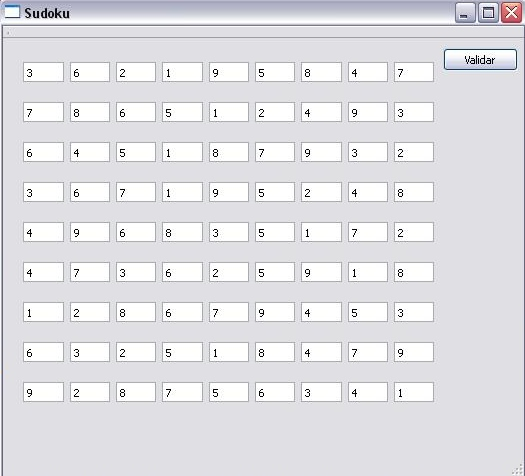
\includegraphics[height=6cm,width=8cm]{sudoku} 


\end{minipage}





\section{Introducción}

Sudoku es un pasatiempo que se publicó por primera vez a finales de la década de 1970 y se popularizó en Japón en 1986, dándose a conocer en el ámbito internacional en 2005 cuando numerosos periódicos empezaron a publicarlo en su sección de pasatiempos. El objetivo del sudoku es rellenar una cuadrícula de 9 x 9 celdas (81 casillas) dividida en subcuadrículas de 3 x 3 (también llamadas "cajas" o "regiones") con las cifras del 1 al 9 partiendo de algunos números ya dispuestos en algunas de las celdas, y lo característico del juego es llenar las casillas vacías con números que no se  repitan en una misma fila, columna o subcuadrícula. \\\\
\begin{center}
		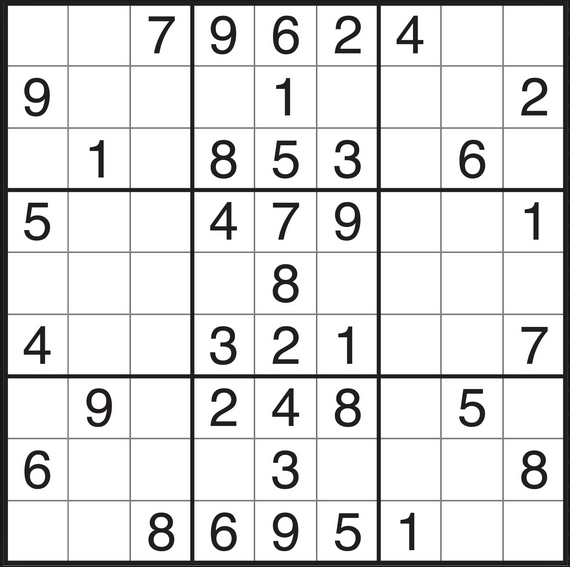
\includegraphics[height=8cm,width=10cm]{sdk.png}
	\end{center}
	
	




\section{Recorriendo Sudoku JCK}

	Nuestro Sudoku muestra en primera instacia la siguiente ventana:
	\begin{center}
		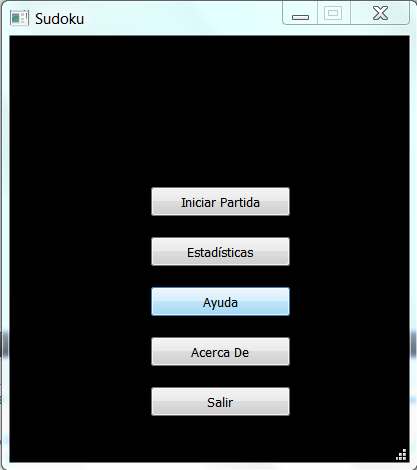
\includegraphics[height=6cm,width=8cm]{ventana_principal.png}
	\end{center}

	\subsection{Iniciar Partida}
		Esta opcion dará inicio a la partida correspondiente a jugar.

	\subsection{Estadísticas}
		Esta opción mostrará el ranking de los jugadores de mejor puntaje en el Sudoku.

	\subsection{Ayuda}
		Aquí se mostrará las reglas y controles necesarios del Sudoku.

	\subsection{Acerca De}
		En esta opción corresponde a la información intelectual del juego.

	\subsection{Salir}
		Como su nombre lo indica, cerrará la aplición.

\section{Recorriendo el Juego.}
	Al haber escogido la opción 'Iniciar Partida', la siguiente ventana de niveles se despliega:
		\begin{center}
			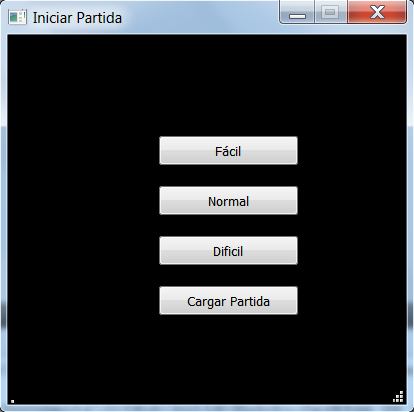
\includegraphics[height=6cm,width=8cm]{ventana_niveles.png}
		\end{center}
	La dificultad se basa en restar la cantidad de números al tablero, la cantidad de casillas blancas son:
		\\Facil   - 
		\\Medio - 
		\\Dificil  - 
		\\Tambien se muestra la opcion 'Cargar Partida' la cual muestra una partida guardada previamente.	
		\\\\Una vez escogido el nivel, aparecerá la ventana del sudoku lista para ser jugada:
		\begin{center}
			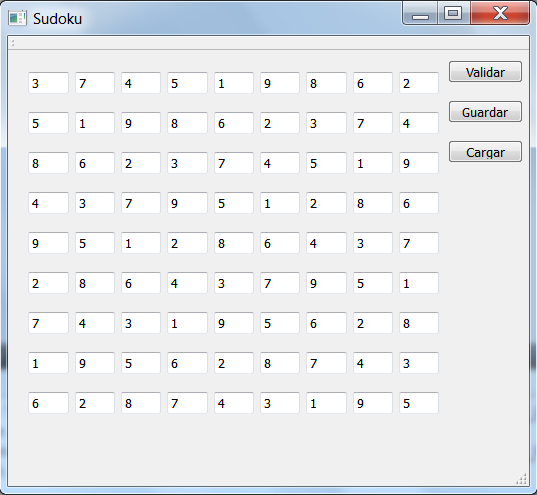
\includegraphics[height=6cm,width=8cm]{ventana_sudoku.png}
		\end{center}



		


\end{document}